\documentclass[11pt, letterpaper]{article}   	% use "amsart" instead of "article" for AMSLaTeX format
\usepackage{graphicx}				% Use pdf, png, jpg, or eps§ with pdflatex; use eps in DVI mode
\usepackage{amssymb}
\usepackage{amsmath}
\usepackage{url}
% Allow inline lists
\usepackage[inline]{enumitem}
\usepackage[backend=biber, style=authoryear, autocite=inline, isbn=false, doi=false, url=false, eprint=false]{biblatex}
% Fix biblatex behavior that writes "In: " before journal name.
\renewbibmacro{in:}{%
  \ifentrytype{article}{}{\printtext{\bibstring{in}\intitlepunct}}}

\newcommand{\floor}[1]{\lfloor #1 \rfloor}
\newcommand{\E}[1]{\left< #1 \right>}
\newcommand{\eq}[1]{Eq.~(\ref{#1})}
\newcommand{\Eq}[1]{Equation~(\ref{#1})}
\newcommand{\eqs}[2]{Eq.~(\ref{#1})~and~(\ref{#2})}
\DeclareMathOperator{\pmi}{pmi}
\DeclareMathOperator{\fpmi}{fpmi}
\DeclareMathOperator{\hilopmi}{hilopmi}


\bibliography{references}

\title{Distinguishing among coalescent models using two-site allele frequency spectra}
\author{Daniel P. Rice}
\date{\today}

\begin{document}
\maketitle

\abstract{[NOTE: OLD]
The genetic diversity of a population reflects its demographic and
evolutionary history. Methods for inferring this history typically
assume that the ancestry of a sample can be modeled by the Kingman
coalescent process. A defining feature of the Kingman coalescent is
that it generates genealogies that are binary trees: no more than two
ancestral lineages may coalesce at the same time. However, this
assumption breaks down under several scenarios. For example, pervasive
natural selection, rapid spatial range expansion, and extreme
variation in offspring number can all generate genealogies with
``multiple-merger'' events in which more than two lineages coalesce
instantaneously. Therefore, detecting multiple mergers is important
both for understanding which forces have shaped the diversity of a
population and for avoiding fitting misspecified models to data.
Current methods to detect multiple mergers rely on the average site
frequency spectrum (SFS). However, the signatures of multiple
mergers in the average SFS are also consistent with a Kingman
coalescent process with a time-varying population size. Here, I
present a new method for detecting multiple mergers based on
the mutual information of the joint allele frequency spectrum at pairs of linked sites. Unlike the average SFS,
the mutual information depends mostly on the topologies of genealogies
rather than their branch lengths and is therefore robust to most
demographic effects.}

\section*{Introduction}
The genetic diversity of a population reflects its demographic and evolutionary history.
Learning about this history from contemporary genetic data is the domain of modern population genetics (see~\cite{Hahn2018a}).
The fundamental tools of the trade are toy models, which are used to study how historical forces shape genetic diversity, and which form the basis of parametric inference methods.
However, populations are complicated and, moreover, varied in their complications.
No simple model can capture the processes governing every species' evolution, and fitting a misspecified model will generate misleading inferences.
It is therefore crucial to understand the limits of our models and to be able to assess when a model is appropriate for a particular data set.

One of the most important and widely used models is the Kingman coalescent~\autocite{Kingman1982a, Kingman1982b, Kingman1982c, Hudson1983, Tajima1983}.
The Kingman coalescent is a stochastic process that generates gene genealogies, trees representing the patterns of shared ancestry of sampled individuals.
Inference methods use these genealogies as latent variables linking demographic parameters to observable data~\autocite{RosenbergNordborg2002}.
The Kingman coalescent has a number of convenient properties that allow for both analytical calculations (e.g.,~\cite{Tajima1989}) and efficient stochastic simulations (e.g.,~\cite{Hudson2002}): tree topologies are independent of waiting times; waiting times are generated by a Markov process; and neutral mutations are modeled as a Poisson process conditionally independent of the tree.
Moreover, the model may be extended to study a variety of biological phenomena including recombination, population structure, and variation in sex ratios or ploidy (see generally~\cite{Wakeley2009}).

In its simplest form, the Kingman coalescent has a single parameter, the coalescent rate, which determines the branch lengths of genealogies~\autocite{Kingman1982a}.
Under a variety of conditions, the coalescent rate is inversely proportional to the size of the population~\autocite{Kingman1982b}.
Accordingly, a growing or shrinking population may be modeled by a time-varying rate~\autocite{GriffithsTavare1994, GriffithsTavare1998}.
This observation is the basis for a variety of methods to infer historical population sizes from genetic data.

With modern population genomics data sets, full-data likelihood models are impractical, so population-size inference is typically done on informative summary statistics.
One widely used statistic is the site frequency spectrum (SFS): the number of mutations observed as a function of their allele frequency in the sample.
The expected number of mutations at a given frequency depends on the branch lengths, and hence, on the coalescent rate.
Thus, one can infer the coalescent rate by integrating over tree topologies, weighted by their probabilities under the Kingman coalescent.
Some methods perform this integration by Monte Carlo simulation (e.g., \cite{CoventryEtAl2010, ExcoffierEtAl2013}).
Others (e.g., \cite{Nielsen2000}, \cite{BhaskarEtAl2015}), compute the expected site frequency spectrum directly for simple demographic models using the results of \cite{GriffithsTavare1998} or \cite{PolanskiKimmel2003}.
(Another class of SFS-based methods are based on corresponding forward-time models rather than the coalescent \autocite{GutenkunstEtAl2009, LukicEtAl2011, RagsdaleGutenkunst2017, JouganousEtAl2017}.)

A serious problem for this inference procedure is that different models of evolution generate different relationships between historical population sizes and genetic diversity.
One of the basic assumptions of the Kingman coalescent is that natural selection is negligible in determining the distribution of genealogies.
When this assumption is violated, Kingman-based inference methods are misspecified.
For example, \cite{SchriderEtAl2016} recently demonstrated how population-size inference can be distorted by selective sweeps.
This effect is present in SFS-based methods as well as in sequentially Markov coalescent methods (e.g., \cite{LiDurbin2011}).
In a similar vein, \cite{CvijovicEtAl2018}, showed that purifying selection at linked sites that is sufficient to reduce overall genetic diversity is also sufficient to distort the SFS, leading to a false signal of population growth.
Genomic evidence from multiple species suggests that such violations of the neutral model underlying the Kingman coalescent may be widespread \autocite{SellaEtAl2009, Corbett-DetigEtAl2015, KernHahn2018}.

An important extension of the Kingman coalescent is a family of models known as \textit{multiple merger coalescents} \autocite{Pitman1999, Sagitov1999, DonnellyKurtz1999,} (reviewed in \cite{Eldon2016}), which arise in a variety of contexts both with and without selection.
Whereas in the Kingman coalescent lineages may coalesce only pairwise, multiple merger coalescents permit more than two lineages to coalesce in a single event.
The even more general class of simultaneous multiple merger coalescents \autocite{Schweinsberg2000, MohleSagitov2001, Sagitov2003} permits more than one multiple merger event at the same time.
These models are relevant for species with
``sweepstakes'' reproductive events \autocite{EldonWakeley2006, SargsyanWakeley2008},
fat-tailed offspring number distributions \autocite{Schweinsberg2003},
recurring selective sweeps at linked sites \autocite{DurrettSchweinsberg2005, CoopRalph},
rapid adaptation \autocite{NeherHallatscheck2013, DesaiEtAl},
and purifying selection at sufficiently dense sites \autocite{Seger, Good, Nicholaisen}.
In each of these contexts, the coalescent timescale is not necessarily proportional to the population size.
For example, with fat-tailed offspring distributions the rate of coalescence is a power law in the population size \autocite{Schweinsberg2003}, while with linked sweeps it is determined by rate of linked sweeps \autocite{DurrettSchweinsberg2005}.
In these settings, interpreting the level of genetic diversity in terms of an ``effective population size'' is misleading and inferences based on the Kingman coalescent may be \emph{qualitatively} incorrect.
It is therefore important to determine whether the Kingman model is appropriate for a given data set before performing demographic inference.

One possible approach to identifying multiple mergers in genomic data is to use the SFS as a summary statistic.
(\cite{Koskela2015} developed a full-likelihood method based on importance sampling, but, as with other ``exact'' inference methods, it does not scale to genomic data.)
\cite{BirknerEtAl2013, BlathEtAl2016, SpenceEtAl2016} derived methods for computing the expected site frequency spectrum of (simultaneous-)multiple merger coalescents.
\cite{EldonEtAl2015} showed that it is possible to distinguish between a multiple merger coalescent of the beta family and the Kingman coalescent with exponential growth using the SFS.
\cite{RodelspergerEtAl2014} detected non-Kingman signatures of widespread linked selection in the nematode \textit{Pristionchus pacificus} by demonstrating that the site frequency spectrum is non-monotonic, a signature of multiple mergers \autocite{NeherHallatscheck2013, BirknerEtAl2013}.

However, existing methods have limitations for distinguishing multiple mergers from general models of population-size change.
The primary signature of multiple mergers in the SFS is an overabundance of low-frequency mutations relative to the Kingman expectation, which is also the signature of population growth.
\cite{EldonEtAl2015} were able to reject exponential growth in favor of multiple mergers with sufficient data, but a more flexible model of growth may be able to fit the multiple mergers SFS (see \cite{MyersEtAl2008, BhaskarSong2014}).
The non-mononotic SFS identified by \cite{RodelspergerEtAl2014} is a more robust signature of multiple mergers, but detecting it in data requires knowledge of the ancestral allele at each site.
High-frequency mutations are typically much rarer than low-frequency mutations, so misidentifying even a small fraction of ancestral alleles can generate a non-monotonic SFS at high frequencies.

Here, we propose that summary statistics based on the spectrum of mutation frequencies at pairs of nearby sites---the 2-SFS \autocite{Hudson2001, FerrettiEtal2018})---are useful for distinguishing between the Kingman coalescent with population growth and multiple merger coalescents.
We show that this is true for both perfectly linked sites and sites separated by a moderate genetic distance.
These statistics may be calculated efficiently from genomic single nucleotide polymorphism data.
Furthermore, they do not require phasing, recombination maps, or ancestral allele identification and are informative even with small sample sizes.
Together, these properties make the 2-SFS useful for demographic model-checking in a wide range of species.
Finally, we demonstrate this model-checking procedure on genomic diversity data from \textit{Drosophila melanogaster} \autocite{LackEtAl2015}.

\section*{Definitions and previously known results}

\subsection*{The SFS and 2-SFS}
Consider a sample of $n$ chromosomes taken from a population of size $N$ with mutation rate $\mu$ per site per generation.
Following the notation of \cite{Fu1995}, the sample site frequency spectrum is $\left\{ \xi_i : 1 \leq i < n \right\}$, where $\xi_i$ is the fraction of sites containing a mutation with derived allele count $i$ in the sample.
In many cases, the ancestral allele is unknown and so the allele in $i$ samples and the complimentary allele in $n-i$ samples are indistinguishable.
Therefore, we will mostly consider the \textit{folded} site frequency spectrum $\left\{ \eta_i = \xi_i + (1-\delta_{i,n-i}) \xi_{n-i}: 1 \leq i \leq \floor{n/2} \right\}$, where $\delta_{k,k'}$ is the Kronecker delta. %, where $\eta_i = \xi_i + \delta_{n-2i} \xi_{n-i}$.

The SFS and folded SFS are single-site statistics.
As such, they can be calculated from a set of single nucleotide polymorphisms (SNPs) without any information about their relative locations in the genome.
We define the two-site frequency spectrum (2-SFS) at distance $d > 0$,
$\left\{ \xi_{ij}(d) : 1 \leq i, j < n\right\}$,
as the fraction of pairs of sites separated by $d$ bases for which there is a mutation with derived allele count $i$ at one site and a second mutation with derived allele count $j$ at the other site.
(Note that $\xi_{ij}(d) = \xi_{ji}(d)$ by symmetry.)
This object has been studied for non-recombining sites by \cite{FerrettiEtAl2018} in a neutral model and \cite{Xie2011} in a model with selection.
By analogy to the folded SFS, we define the folded 2-SFS, as
\begin{align*}
    \eta_{ij}(d) &= \xi_{ij}(d) \\
                 &+ (1-\delta_{i,n-i}) \xi_{n-i,j}(d) \\
                 &+ (1-\delta_{j,n-j}) \xi_{i,n-j}(d) \\
                 &+ (1-\delta_{i,n-i}) (1-\delta_{j,n-j}) \xi_{n-i,n-j}(d).
\end{align*}
In this section, we will be considering non-recombining sites and so will suppress the distance $d$.

In the limit of low per-site mutation rate ($\mu\to0$), all polymorphic sites are bi-allelic and the expected SFS and 2-SFS are related to moments of the branch length distribution by
\begin{align}
    \E{\xi_i} &= \mu \E{\tau_i} \label{eq:expected_sfs} \\
    \E{\xi_{ij}} &= \mu^2 \E{\tau_i \tau_j},
    \label{eq:expected_2sfs}
\end{align}
where $\tau_i$ is the total length of branches subtending $i$ leaves of a gene genealogy and $\E{\cdot}$ represents the expectation over the distribution of gene genealogies defined by a coalescent model.
Thus, the SFS and 2-SFS depend on the distribution of coalescent times as well as the distribution of tree topologies.

\cite{Fu1995} calculated the first and second moments of the branch-length distribution for non-recombining infinite sites locus under the standard time-homogeneous Kingman coalescent.
He found that $\E{\tau_i \tau_j} < \E{\tau_i}\E{\tau_j}$ for all $j \neq i, (n-i)$.
This result, combined with \eqs{eq:expected_sfs}{eq:expected_2sfs}, implies a negative correlation between mutations at different frequencies: trees generating a mutation with derived allele count $i$ are less likely than average to generate a second mutation with derived allele count $j \neq i, (n-i)$.
(There are positive correlations between mutations at complimentary frequencies induced by genealogies whose root node partitions the tree into subtrees of size $i$ and $n-i$.)

\cite{BirknerEtAl2013} extended Fu's calculation to a family of multiple merger coalescents called beta coalescents.
This one-parameter family interpolates between the Kingman coalescent and the Bolthausen-Sznitman coalescent as the parameter, $\alpha$, varies from 2 to 1.
Beta coalescents arise in models with fat-tailed offspring distributions \autocite{Schweinsberg2003}, and the Bolthausen-Sznitman coalescent is the limiting distribution of genealogies in rapidly adapting populations \autocite{NeherHallatscheck2013}.
Like Fu, Birkner et al.\ were primarily concerned with computing the sample variance of SFS-based summary statistics such as Tajima's D \autocite{Tajima1989}.
As a result, they were mostly interested in the diagonal terms of the SFS covariance matrix, which dominate that calculation.
However, Figures 5 and 6 of \cite{BirknerEtAl2013} show positive correlations between $\xi_i$ and $\xi_j$ for $j \neq i, n-i$.
Thus, unlike the standard Kingman coalescent, the beta coalescent can generate positive associations between mutations with different minor allele counts.

Our goal is to demonstrate that this distinction in the 2-SFS between the multiple merger and Kingman coalescents
\begin{enumerate*}[label=(\roman*), before=\unskip{: }, itemjoin={{; }}, itemjoin*={{, and }}]
    \item applies to Kingman coalescents with time-varying coalescent rates
    \item is robust to recombination between the sites
    \item is also a feature of forward-time models with selection
    \item can form the basis of a model-checking procedure for demographic inference methods
\end{enumerate*}.
To this end, we will make use of the fact that the 2-SFS may be interpreted as a joint probability distribution to define the following useful transformation.

\subsection*{Frequency pointwise mutual information}

Given a coalescent model, the minor allele count at an arbitrary site is a random variable with probability mass function $p(i) = \E{\eta_i}$, where we define $\eta_0$ to be the fraction of monomorphic sites.
Similarly, the minor allele counts at a pair of sites separated by $d$ bases is a pair of random variables with joint probability mass function $p_d(i,j) = \E{\eta_{ij}(d)}$.
We are interested in quantifying the dependence between minor allele counts at a given pair of sites, particularly for $i\neq j$.

A general measure of the dependence between a pair of random variables is the \textit{mutual information} \autocite{CoverThomas1991}.
The mutual information between random variables $X$ and $Y$ is a functional of their joint probability mass function, $p(x,y)$, defined as
\begin{align}
    I[p(x,y)] = \sum_{x,y} p(x,y) \log \frac{p(x,y)}{p(x)p(y)},
    \label{eq:mutual_information}
\end{align}
where, with slight abuse of notation, $p(x) = \sum_y p(x,y)$ and vice versa.
Equivalently, the mutual information is the Kullback-Leibler divergence between the true joint distribution of $X$ and $Y$ and the joint distribution of two independent random variables with the same marginal distributions as $X$ and $Y$ \autocite{CoverThomas1991}.
Thus, mutual information captures generic, possibly nonlinear, dependence between $X$ and $Y$.

We would like to measure the association between alleles at particular frequencies, rather than the overall dependence between allele frequencies at nearby sites (which would be a measure of linkage disequilibrium).
\Eq{eq:mutual_information} shows that $I[p(x,y)]$ is the expectation, relative to $p(x,y)$, of a quantity known as the \textit{pointwise mutual information}, where
\begin{align}
    \pmi(x,y) = \log \frac{p(x,y)}{p(x)p(y)} = \log \frac{p(x|y)}{p(x)} = \log \frac{p(y|x)}{p(y)}
\end{align}
\autocite{ChurchHanks1990}.
Pointwise mutual information measures the change in the probability that $X=x$ given knowledge that $Y=y$.
When $X$ and $Y$ are independent, $\pmi(x,y) = 0$ for all $x,y$.
On the other hand, when $X$ and $Y$ are not independent, $\pmi(x,y) > 0$ implies that $p(x|y) > p(x)$, and conversely for $\pmi(x,y) < 0$.

As we have shown above, the expected folded 2-SFS is a joint probability mass function over minor allele counts.
We may thus define the \textit{frequency pointwise mutual information} as
\begin{align}
    \fpmi(i,j;d) = \log \frac{\E{\eta_{i,j}(d)}}{\E{\eta_i} \E{\eta_j}}.
\end{align}
This transformation of the 2-SFS has several useful properties.
First, because it is based on the minor allele frequencies, we may compute $\fpmi$ from data without knowing the ancestral allele.
Moreover, the results of \cite{Fu1995} show that $\fpmi(i,j) < 0$ for $i\neq j$ for non-recombining sites under the time-homogeneous Kingman coalescent.

The second benefit of computing $\fpmi$ from the 2-SFS is that it normalizes for distortions in the SFS.
Population-size variation distorts the SFS by changing the distribution of waiting times.
However, the time-inhomogeneous Kingman coalescent generates the same distribution of tree topologies as the time-homogeneous version.
On the other hand, multiple mergers alter both the coalescent time distribution and the distribution of topologies.
These two effects are convolved in the SFS, making it difficult to distinguish between population growth and multiple mergers.
Our hope is that the 2-SFS contains additional information about the distribution of genealogies, once distortions in coalescent times are accounted for.

\subsection*{Coarse-grained frequencies}

With finite data, estimates of the 2-SFS will be noisy.
This is particularly true for $i,j\gg1$ because $\E{\eta_{ij}}$ decays like $(ij)^{-1}$ for the standard Kingman \autocite{Fu1995} and faster with growth or multiple mergers.
We show in Results that a positive association between mutations with high minor allele counts and mutations with low minor allele counts is a signature of multiple mergers.
This suggests a coarse-grained SFS and 2-SFS:
\begin{align}
    \eta_{\text{lo}}(i_c) &= \sum_{i=1}^{i_c-1} \eta_i \\
    \eta_{\text{hi}}(i_c) &= \sum_{i=i_c}^{\floor{n/2}} \eta_i \\
    \eta_{\text{hi,lo}}(d; i_c) &= \sum_{i=1}^{i_c-1} \sum_{j=i_c}^{\floor{n/2}} \eta_{ij}(d),
\end{align}
where $i_c$ is an arbitrary cutoff between high and low minor allele frequency.
Coarse-graining allows us to estimate the 2-SFS stably for large sample sizes, because we may adjust $i_c$ to ensure a large number of sites in both the high--minor allele count and low--minor allele count bins.

We can also compute the pointwise mutual information in this coarse-grained distribution as
\begin{align}
    \hilopmi(d; i_c) = \log \frac
                                {\E{\eta_{\text{hi,lo}}(d; i_c)}}
                                {\E{\eta_{\text{lo}}(i_c)}  \E{\eta_{\text{hi}}(i_c)}}.
\end{align}
One could similarly calculate five other pointwise mutual information statistics from the coarse-grained 2-SFS (e.g., the PMI between monomorphic sites and sites with high minor allele counts), but we will not use these statistics here.

\section*{Results \label{sec:results}}

\subsection*{Population growth vs. the beta coalescent in non-recombining loci}

\begin{itemize}
    \item Want to calculate PMI for 2-SFS for various models.
    \item implemented Fu and Birkner formulas
    \item \cite{ZivkovicWiehe2008} extended Fu to variable population size.
    \item We implemented their formula for exponential growth and piecewise constant, but in principle could be extended to other models.
    \item Figure 1 shows weighted PMI $\text{wPMI}(i,j) = \E{\eta_{ij}} \text{PMI}(i,j)$.
    \item weighted to highlight regions of the 2-SFS with the most mutations.
    \item Observations:
    \begin{enumerate}
        \item population growth does not qualitatively change the PMI, even though it distorts the SFS a lot.
        \item more multiple mergers leads more positive elements.
        \item Positive associations off-diagonal. Presumably due to uneven branching. Going to ignore because turns out to be sensitive to recombination.
        \item Positive associations between high- and low-frequency mutations. This is the signal we'll focus on.
    \end{enumerate}
    \item Suggests a coarse-graining of the SFS into high- and low-frequency mutations.
    \item Definition of hi-lo corr given cutoff and distance.
\end{itemize}

[Next: Intuition and $n=4$ calculations.]

% \begin{figure}
% \centering
% 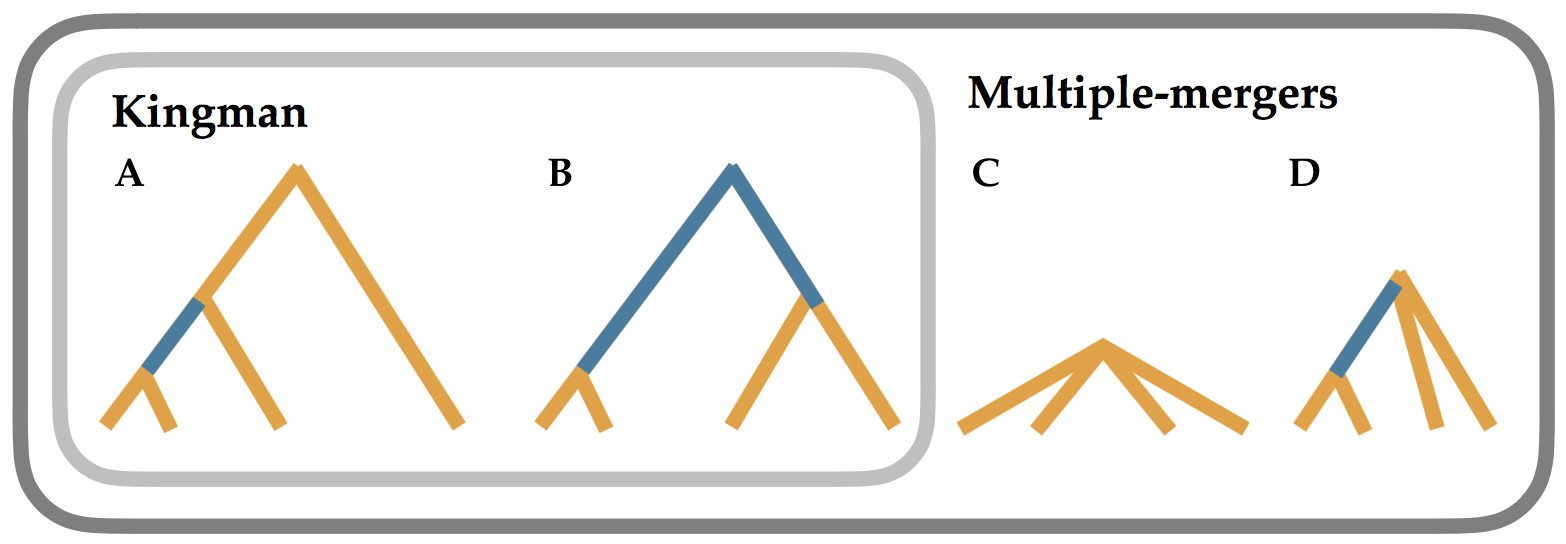
\includegraphics[width=0.8\textwidth]{figures/trees.png}
% \caption{Possible genealogies with a sample size of $n=4$. Opportunities for singleton/tripleton mutations are in orange. Opportunities for doubletons are in blue.  \label{fig:trees}}
% \end{figure}
%
% We can get an intuitive understanding for this result by considering a sample of size 4. In the Kingman coalescent, there are only two possible tree topologies (\Fig{fig:trees}).
% Furthermore, the total branch length is independent of the topology.
% As a result, there is a trade-off between the branch length leading to singleton/tripleton mutations and the branch length leading to doubletons: loci with topology (A) will have more opportunities for the former and loci with topology (B) will have more opportunities for the latter.
% Conditional on observing a doubleton at a locus, it is thus more likely that the locus has topology (B) and so the expected number of singletons is lower.
% In terms of the joint site frequency spectrum, we have $\E{\phi_{12}} < \E{\phi_{1}} \E{\phi_{2}}$.
%
% On the other hand, multiple mergers induce correlations between the tree topology and the total branch length.
% For example, topology (C) has less overall opportunity for singletons as well as doubletons than (A) or (B), even though the expected proportion of singletons is higher.
% Thus, observing \emph{any mutation at all} makes topology (C) less likely and the expected number of other mutations at all frequencies more likely.
% If multiple-mergers events are frequent enough, this effect may dominate the tradeoff between (A) and (B) and lead to $\E{\phi_{12}} > \E{\phi_{1}} \E{\phi_{2}}$.
%
% There are two limitations of these existing results.
% First, they only apply to time-homogeneous coalescent processes and thus do not distinguish between multiple-mergers coalescents and Kingman models with time-varying population size.
% Second, they assume a non-recombining locus and may break down for sites separated by a finite genetic distance.

\subsection*{Pointwise mutual information between recombining sites}
[Coalescent simulations with recombination (it still works).]

\subsection*{Linked selective sweeps}
[Forward-time simulations of linked sweeps (still works).]

\subsection*{Application to \textit{Drosophila melanogaster}}

\section*{Discussion}
\begin{itemize}
    \item Focus here on coalescent, but also relevant for diffusion methods
    \item Single-locus tests that rely on trees (Seger whale lice, Neher with viruses)
    \item Multi-locus tests that compare vs genomic background
    \item Could extend to a local method to look for variation in ``multiple-merger-ness''
    \item Could also extend
\end{itemize}

Tests of the standard Kingman coalescent based on the SFS originated with \cite{Tajima1989}, \cite{FuLi1993}, and \cite{SimonsenEtAl1995} (see \cite{Achaz2009} for a unifying framework).

\section*{Methods}
\begin{itemize}
    \item Code to compute moments
    \item Simulation code extending msprime
    \item Forward-time simulation with SLiM
    \item Drosophila
    \begin{itemize}
        \item data pre-processing
        \item fitting demographic model with fastNeutrino
        \item simulating demographic model (could maybe compute exactly)
    \end{itemize}
\end{itemize}

\printbibliography

\end{document}
